\section{Sở GD\&ĐT Quảng Ninh 25--26, Lần 1}
\Opensolutionfile{ans}[ans/ans-11-26-2-QuangNinh-SoGD-L1-LC]
\caulc
\begin{ex}%[1D6N4-2]
Nghiệm của phương trình $\log_3(x+1)=2$ là 
\choice
{$x=6$}
{$x=5$}
{\True $x=8$}
{$x=10$}
\loigiai{Điều kiện xác định $x>-1$.
\begin{eqnarray*}
& &\log_3(x+1)=2\\
&\Leftrightarrow&x+1=3^2\\
&\Leftrightarrow&x=8.
\end{eqnarray*}
So với điều kiện, phương trình có nghiệm là $x=8$.}
\end{ex}
\begin{ex}%[2D1N2-2]
Cho hàm số $y=f(x)$ liên tục trên $\mathbb{R}$ và có bảng xét dấu của $f'(x)$ như sau\\
\begin{center}

\begin{tikzpicture}
\tkzTabInit[nocadre=false,lgt=1.2, espcl=1.5,deltacl=0.5]
{$x$ / 1 , $f'(x)$ / 1} 
{$-\infty$, $-1$, $0$, $1$, $2$, $+\infty$} 
\tkzTabLine{, +, 0, -, 0, +, d, -, 0, -, }
\end{tikzpicture}
\end{center}
Số điểm cực đại của hàm số $y=f(x)$ là 
\choice
{$1$}
{\True $2$}
{$3$}
{$4$}
\loigiai{Dựa vào bảng xét dấu của $y=f'(x)$. Ta thấy, hàm số $y=f(x)$ có $2$ điểm cực đại.}
\end{ex}
\begin{ex}%[1H8H7-1]
Cho hình chóp tứ giác đều $S.ABCD$ có độ dài cạnh đáy là $\sqrt{2}$ và tam giác $SAC$ đều. Độ dài cạnh bên của hình chóp đã cho bằng 
\choice
{\True $2$}
{$\sqrt{2}$}
{$1$}
{$\sqrt{3}$}
\loigiai{
\immini{Xét hình vuông $ABCD$ có đường chéo là $AC$ nên $AC=\sqrt{2}\cdot \sqrt{2}=2$.\\
Mặt khác, tam giác $SAC$ là tam giác đều cạnh $SA=AC=2$. }
{\begin{tikzpicture}[scale=1,>=stealth,line join=round,line cap=round]
\draw[dashed,black,scale=2.5] (0,0)coordinate(A)--(-130:0.5)coordinate(B)--(1,0)coordinate(D)--(A)--($(D)-(A)+(B)$)coordinate(C);
\path[name path=dtAC] (A)--(C);
\path[name path=dtBD] (B)--(D);
\path[name intersections={of= dtAC and dtBD}] coordinate(O)at(intersection-1);
\draw[dashed,black,scale=2.5] (O)--($(O)+(90:1)$)coordinate(S)--(A);
\draw[black,scale=2.5] (S)--(B)--(C)--(D)--(S)--(C);
\path[scale=2.5] pic[angle radius=5,draw=blue,angle eccentricity=1.5] {right angle = S--O--B};
\foreach \diem/\vitrin in {S/above,A/above right,B/below left,C/below right,D/right,O/below} \fill (\diem)circle(1.5pt)node[\vitrin]{$\diem$};
\end{tikzpicture}}}
\end{ex}
\begin{ex}%[2H5N1-3]
Trong không gian với hệ trục tọa độ $Oxyz$, mặt phẳng đi qua $M(1;2;-4)$ và vuông góc với trục $Oz$ có phương trình là 
\choice
{$x+2y-4z-21=0$}
{\True $z=-4$}
{$z=4$}
{$x+2y+4z-21=0$}
\loigiai{
Vì mặt phẳng vuông góc với trục $Oz$ nên nhận $\overrightarrow{k}=(0;0;1)$ làm vectơ pháp tuyến và qua $M(1;2;-4)$. Khi đó, mặt phẳng cần tìm là $z+4=0$ hay $z=-4$.}
\end{ex}
\begin{ex}%[1H8H6-1]
Cho hình lăng trụ đứng $ABC.A'B'C'$ có tất cả các cạnh bằng $1$. Góc tạo bởi đường thẳng $A'C$ và mặt phẳng $(ABC)$ bằng 
\choice
{\True $45^{\circ}$}
{$90^{\circ}$}
{$60^{\circ}$}
{$30^{\circ}$}
\loigiai{
\immini{
Ta có $AA'\perp (ABC)\Rightarrow A$ là hình chiếu vuông góc của $A'$ lên $(ABC)$.\\
Suy ra, $AC$ là hình chiếu vuông góc của $A'C$ lên $(ABC)$.\\
Suy ra, $\left(A'C,(ABC)\right)=\left(A'C,AC\right)=\widehat{ACA'}$.\\
Mặt khác, tứ giác $AA'C'C$ là hình vuông nên $\widehat{ACA'}=45^{\circ}$.
}
{\begin{tikzpicture}[>=stealth,line join=round,line cap=round]
\draw[black,scale=2.5] (0,0)coordinate(A)--(-35:0.8)coordinate(B)--(1,0)coordinate(C)--($(C)+(90:1)$)coordinate(C')--($(B)-(C)+(C')$)coordinate(B')--($(A)-(B)+(B')$)coordinate(A')--(C') (A)--(A') (B)--(B');
\draw[dashed,black,scale=2.5] (A)--(C);
\foreach \diem/\vitrin in {A/left,B/below left,C/right,A'/left,B'/below left,C'/right}	\fill (\diem)circle(1.5pt)node[\vitrin]{$\diem$};
\end{tikzpicture}
}
}
\end{ex}
\begin{ex}%[1D1N4-6]
Tập giá trị của hàm số $y=3\cos 2x$ là 
\choice
{$T=[-6;6]$}
{\True $T=[-3;3]$}
{$T=\mathbb{R}$}
{$T=[-2;2]$}
\loigiai{
Tập xác định $\mathscr{D}=\mathbb{R}$.\\
Ta có
\begin{align*}
&-1\leq \cos 2x\leq 1,\,\forall x\in \mathbb{R}\\
\Leftrightarrow& -3\leq 3\cos 2x\leq 3,\,\forall x\in \mathbb{R}.
\end{align*}
Vậy tập giá trị là $T=[-3;3]$.
}
\end{ex}
\begin{ex}%[2D4N1-2]
Họ nguyên hàm của hàm số $f(x)=x-\dfrac{1}{x^2}$ là 
\choice
{\True $\dfrac{1}{2}x^2+\dfrac{1}{x}+C$}
{$1+\dfrac{1}{x}+C$}
{$x+\dfrac{1}{x}+C$}
{$\dfrac{1}{2}x^2-\dfrac{1}{x}+C$}
\loigiai{
Ta có $\displaystyle\int \left(x-\dfrac{1}{x^2}\right)\mathrm{\,d}x=\dfrac{1}{2}x^2+\dfrac{1}{x}+C$.}
\end{ex}
\begin{ex}%[1D2H3-2]
Cho cấp số nhân $(u_n)$ với $u_1=2$ và $u_3=162$. Giá trị của công bội $q$ bằng 
\choice
{$q=\dfrac{1}{3}$}
{\True $q=\pm3$}
{$q=3$}
{$q=\pm\dfrac{1}{3}$}
\loigiai{
Áp dụng công thức số hạng tổng quát của cấp số nhân. Ta có
\begin{eqnarray*}
& &u_3=u_1\cdot q^2\\
&\Leftrightarrow&q^2=\dfrac{162}{2}\\
&\Leftrightarrow& q^2=9\\
&\Leftrightarrow& q=\pm 3.
\end{eqnarray*}}
\end{ex}
\begin{ex}%[2H5N3-3]
Trong không gian với hệ trục tọa độ $Oxyz$, cho các điểm $A(1;1;2)$, $B(3;2;-3)$. Phương trình mặt cầu $(S)$ có tâm $A$ và đi qua điểm $B$ là 
\choice
{\True $(x-1)^2+(y-1)^2+(z-2)^2=30$}
{$(x+1)^2+(y+1)^2+(z+2)^2=30$}
{$(x-1)^2+(y-1)^2+(z-2)^2=\sqrt{30}$}
{$(x+1)^2+(y+1)^2+(z+2)^2=\sqrt{30}$}
\loigiai{
Phương trình mặt cầu $(S)$ có tâm $A(1;1;2)$ và bán kính $R=AB=\sqrt{30}$.
\[(x-1)^2+(y-1)^2+(z-2)^2=30.\]}
\end{ex}
\begin{ex}%[1D5N2-3]
Doanh thu bán hàng trong $20$ ngày của một cửa hàng được ghi lại ở bảng sau (đơn vị: triệu đồng)
\begin{center}
\begin{tabular}{|l|c|c|c|c|c|}
\hline
Doanh thu & $[5;7)$ & $[7;9)$ & $[9;11)$ & $[11;13)$ & $[13;15)$ \\
\hline
Số ngày & $2$ & $7$ & $7$ & $3$ & $1$ \\
\hline
\end{tabular}
\end{center}
Tứ phân vị thứ ba của mẫu số liệu trên gần nhất với giá trị nào trong các giá trị sau? 
\choice
{$13$}
{$12$}
{\True $11$}
{$10$}
\loigiai{
Bảng xử lý số liệu
\begin{center}
\begin{tabular}{|l|c|c|c|c|c|}
\hline
Doanh thu & $[5;7)$ & $[7;9)$ & $[9;11)$ & $[11;13)$ & $[13;15)$ \\
\hline
Số ngày & $2$ & $7$ & $7$ & $3$ & $1$ \\
\hline
Tần số tích lũy & $2$ & $9$ & $16$ & $19$ & $20$ \\
\hline
\end{tabular}
\end{center}
Tổng tần số $n=20$.\\
Xét $\dfrac{3\cdot 20}{4}=15\leq 16$. Suy ra, nhóm $3$ chứa $Q_3$.\\
Giá trị $Q_3=9+\dfrac{15-9}{7}\cdot 2=\dfrac{75}{7}\approx 11$.
}
\end{ex}
\begin{ex}%[2D4N3-4]
Trong không gian với hệ trục tọa độ $Oxyz$, một vật thể nằm giữa hai mặt phẳng $x=a$; $x=b$ với $a < b$, thiết diện của vật thể bị cắt bởi mặt phẳng vuông góc với trục $Ox$ tại điểm có hoành độ $x\,(a\le x\le b)$ là một hình phẳng có diện tích bằng $S(x)$, $S(x)$ là một hàm liên tục trên $[a;b]$. Thể tích vật thể được tính bằng công thức 
\choice
{$\pi\displaystyle\int\limits_a^b S(x)\mathrm{\,d}x$}
{$\pi\displaystyle\int\limits_a^b(S(x))^2\mathrm{\,d}x$}
{$\displaystyle\int\limits_a^b(S(x))\mathrm{\,d}x$}
{\True $\displaystyle\int\limits_a^b S(x)\mathrm{\,d}x$}
\loigiai{
Trong không gian với hệ trục tọa độ $Oxyz$, một vật thể nằm giữa hai mặt phẳng $x=a$; $x=b$ với $a < b$, thiết diện của vật thể bị cắt bởi mặt phẳng vuông góc với trục $Ox$ tại điểm có hoành độ $x\,(a\le x\le b)$ là một hình phẳng có diện tích bằng $S(x)$, $S(x)$ là một hàm liên tục trên $[a;b]$. Thể tích vật thể được tính bằng công thức 
\[V=\displaystyle\int\limits_a^b S(x)\mathrm{\,d}x.\]}
\end{ex}
\begin{ex}%[2H2N1-1]
Cho tứ diện $ABCD$. Gọi $M, N$ lần lượt là trung điểm của $AD$ và $BC$. Tổng $\overrightarrow{AB}+\overrightarrow{DC}$ bằng 
\choice
{$\overrightarrow{0}$}
{$2\overrightarrow{NM}$}
{$2\overrightarrow{AD}$}
{\True $2\overrightarrow{MN}$}
\loigiai{
\immini{
Ta có
\begin{itemize}
\item $\overrightarrow{AB}=\overrightarrow{AM}+\overrightarrow{MN}+\overrightarrow{NB}$.
\item $\overrightarrow{DC}=\overrightarrow{DM}+\overrightarrow{MN}+\overrightarrow{NC}$.
\end{itemize}
Khi đó,
\begin{align*}
\overrightarrow{AB}+\overrightarrow{DC}&=\overrightarrow{AM}+\overrightarrow{MN}+\overrightarrow{NB}+\overrightarrow{DM}+\overrightarrow{MN}+\overrightarrow{NC}\\
&=(\overrightarrow{AM}+\overrightarrow{DM})+(\overrightarrow{NB}+\overrightarrow{NC})+2\overrightarrow{MN}\\
&=\overrightarrow{0}+\overrightarrow{0}+2\overrightarrow{MN}\\
&=2\overrightarrow{MN}.
\end{align*}
Vì $m$, $N$ lần lượt là trung điểm $AD$ và $BC$ nên $\overrightarrow{AM}+\overrightarrow{DM}=\overrightarrow{0}$ và $\overrightarrow{NB}+\overrightarrow{NC}=\overrightarrow{0}$.
}{\begin{tikzpicture}[>=stealth,line join=round,line cap=round]
\draw[black,scale=2.5] (0,0)coordinate(B)--(-35:0.8)coordinate(C)--(1,0)coordinate(D);
\draw[dashed,black,scale=2.5] ($(C)!.5!(D)$)coordinate(M1) ($(B)!2/3!(M1)$)coordinate(H) (B)--(D) ($(H)+(90:1)$)coordinate(A);
\draw[black,scale=2.5] (B)--(A)--(D) (A)--(C);
\path ($(A)!0.5!(D)$) coordinate (M);
\path ($(B)!0.5!(C)$) coordinate (N);
\foreach \diem/\vitrin in {A/above,B/left,C/below left,D/right,M/right,N/left}	\fill (\diem)circle(1.5pt)node[\vitrin]{$\diem$};
\end{tikzpicture}}}
\end{ex}
\Closesolutionfile{ans}

\cauds
\Opensolutionfile{ans}[ans/ans-11-26-2-QuangNinh-SoGD-L1-DS]
\begin{ex}%[2D6V1-3]
Trong một cuộc thi Olympic môn Toán dành cho học sinh THPT, trường THPT A có $51$ học sinh và trường THPT B có $24$ học sinh tham dự. Giả sử xác suất giành huy chương vàng của mỗi học sinh của trường A và B lần lượt là $0{,}08$ và $0{,}06$. Chọn ngẫu nhiên một học sinh trong số các học sinh tham dự.
\choiceTF
{\True Xác suất để học sinh được chọn thuộc trường A là $\dfrac{17}{25}$}
{Biết rằng học sinh được chọn thuộc trường B, xác suất để học sinh đó không giành được huy chương vàng là $0{,}92$}
{Xác suất để học sinh được chọn giành huy chương vàng là $\dfrac{48}{625}$}
{\True Biết rằng học sinh được chọn giành huy chương vàng, xác suất để học sinh đó thuộc trường A là $\dfrac{17}{23}$}
\loigiai{
Gọi các biến cố sau
\begin{itemize}
\item A là biến cố \lq\lq Học sinh được chọn học trường A\,\rq\rq.
\item B là biến cố \lq\lq Học sinh được chọn đạt huy chương vàng\,\rq\rq.
\end{itemize}
\begin{center}
\begin{tikzpicture}[
level distance=2.5cm, 
level 1/.style={sibling distance=5cm},
level 2/.style={sibling distance=2.5cm},
every node/.style={draw, rectangle, rounded corners, inner sep=5pt},
label node/.style={
draw=none, 
font=\small, 
midway, 
fill=white, % Quan trọng: tạo nền trắng che đường kẻ
inner sep=2pt}]
\node {Gốc}
child { node {$A$}
child { node {$B$} 
edge from parent node[label node] {$0{,}08$}}
child { node {$\overline{B}$} 
edge from parent node[label node] {$0{,}92$}}
edge from parent node[label node] {$\dfrac{17}{25}$}}
child { node {$\over{A}$}
child { node {$B$} 
edge from parent node[label node] {$0{,}06$}}
child { node {$\overline{B}$} 
edge from parent node[label node] {$0{,}94$}}
edge from parent node[label node] {$\dfrac{8}{25}$}};
\end{tikzpicture}
\end{center}
\begin{itemchoice}
\itemch 
Tổng số học sinh 2 trường là $51+24=75$ (học sinh).\\
Xác suất đề học sinh được chọn thuộc trường A là $\mathrm{P}(A)=\dfrac{51}{75}=\dfrac{17}{25}$.
\itemch 
Ta tính $\mathrm{P}(\overline{B}|\overline{A})=0{,}94$.
\itemch 
Xác suất học sinh đạt huy chương vàng là 
\[\mathrm{P}(B)=\dfrac{17}{25}\cdot 0{,}08+\dfrac{8}{25}\cdot 0{,}06=\dfrac{46}{625}.\]
\itemch 
Ta tính $\mathrm{P}(A|B)=\dfrac{\dfrac{17}{25}\cdot 0{,}08}{\dfrac{46}{625}}=\dfrac{17}{23}$.
\end{itemchoice}
}
\end{ex}
\begin{ex}%[2D4V3-3]
\immini{
Bút viết của một bảng vẽ điện tử được để trong một chiếc giá là một khối tròn xoay có mặt cắt qua trục là một hình phẳng có hình dạng và các kích thước gắn với hệ trục tọa độ $Oxy$ như hình vẽ dưới đây
Biết biên của mặt cắt gồm hai nửa đường tròn đường kính $AB$, $CD$ và một cung của parabol đỉnh $O$, nhận $Ox$ là trục đối xứng; cho $AB=CD=3$ (cm), $OI=1$ (cm), $AD=3$ (cm), $MN=2$ (cm), đơn vị trên hệ trục là $1$ cm.
}{
	\begin{tikzpicture}[>=Stealth, scale=0.6]
		\draw[step=1, gray!20, thin] (-3.5,-4.5) grid (3.5,4.5);
		\draw[->, thick] (-3.5,0) -- (4,0) node[below] {$x$};
		\draw[->, thick] (0,-4.5) -- (0,4.5) node[left] {$y$};
		\coordinate (A) at (-2,2); \coordinate (B) at (2,2);
		\coordinate (C) at (2,-2); \coordinate (D) at (-2,-2);
		\coordinate (I) at (-2,0); \coordinate (M) at (2,1);
		\coordinate (N) at (2,-1); \coordinate (O) at (0,0);
		\draw[thick] (A) -- (D) (B) -- (M) (N) -- (C);
		\draw[dashed] (A) -- (B) (D) -- (C);
		\draw[very thick, green!40!black] (A) arc (180:0:2);
		\draw[very thick, purple!70!black] (D) arc (180:360:2);
		\draw[very thick, blue!60] plot[domain=-1:1, samples=100] ({2*\x*\x}, {\x});
		\foreach \p/\pos/\txt/\col in {
			A/left/A/blue, 
			B/right/B/blue, 
			I/above left/I/blue, 
			O/below left/O/blue, 
			M/right/M/blue, 
			N/right/N/blue, % Điểm N đã được đổi thành Blue
			D/left/D/gray, 
			C/right/C/gray%
		} {
			\fill[\col!80, draw=black!50] (\p) circle (2.5pt);
			\node[\pos] at (\p) {$\txt$};}
	\end{tikzpicture}
	
}
\choiceTF
{\True Phương trình của parabol là $y^2=\dfrac{1}{2} x$}
{Diện tích mặt cắt (làm tròn tới hàng đơn vị) là $14$ (cm$^2$)}
{\True Thể tích phần lõm của giá để bút được tính bằng công thức $\pi \displaystyle\int\limits_0^2\dfrac{1}{2} x\, \mathrm{d}x$}
{Thể tích của toàn bộ giá để bút (làm tròn tới hàng phần chục) bằng $65{,}4$ (cm$^3$)}
\loigiai{
\begin{itemchoice}
\itemch 
Gọi parabol địa diện cho đường cong $MNP$ là $(P)\colon y^2=2px$.\\
Vì $(P)$ qua $N(2;1)$ nên $4p=1\Leftrightarrow p=\dfrac{1}{4}$.\\
Vậy $(P)\colon y^2=\dfrac{1}{2}x$.
\itemch 
Diện tích hình tròn được ghép từ hai nửa là
\[S_1=\pi\cdot \left(\dfrac{AB}{2}\right)^2=\pi\cdot \left(\dfrac{3}{2}\right)^2=\dfrac{9}{4}\pi\,(\text{cm}^2).\]
Diện tích hình vuông $ABCD$ là
\[S_2=3^2=9\,(\text{cm}^2).\]
Diện tích parabol $MON$ là
\[S_3=2\cdot \displaystyle\int\limits_0^2 \sqrt{\dfrac{1}{2}x}\mathrm{\,d}x=\dfrac{8}{3}\,(\text{cm}^2).\]
Diện tích mặt cắt là
\[S=S_1+(S_2-S_3)=\dfrac{9}{4}\pi+\left(9-\dfrac{8}{3}\right)\approx 13\,(\text{cm}^2).\]
\itemch 
Thể tích lõi parabol là
\[V_1=\pi\displaystyle\int\limits_0^2 y^2\mathrm{\,d}x=\pi\displaystyle\int\limits_0^2 \dfrac{1}{2}x\mathrm{\,d}x.\]
\itemch 
Phương trình đường tròn đường kính $AB$ có tâm là $(0;2)$ và bán kính là $2$.
\[x^2+(y-2)^2=2^2\Rightarrow y=2+\sqrt{4-x^2}.\]
Thể tích nửa giá bút (phần bên trái trục $Oy$)
\[V=\pi\displaystyle\int\limits_{-2}^2 \left(2+\sqrt{4-x^2}\right)^2\mathrm{\,d}x-V_1=\pi\displaystyle\int\limits_{-2}^2 \left(2+\sqrt{4-x^2}\right)^2\mathrm{\,d}x-\pi\displaystyle\int\limits_0^2 \dfrac{1}{2}x\mathrm{\,d}x\approx159{,}6\,(\text{cm}^3).\]
\end{itemchoice}}
\end{ex}
\begin{ex}%[2H5H3-2]
Trong không gian với hệ trục tọa độ $Oxyz$, cho các điểm $A(-2; 0; 0)$, $B(0;-2; 0)$, $C(0; 0;-2)$. Điểm $D$ khác gốc tọa độ sao cho $DA$, $DB$, $DC$ đôi một vuông góc.
\choiceTF
{\True Mặt phẳng $(ABC)$ có phương trình $\dfrac{x}{2}+\dfrac{y}{2}+\dfrac{z}{2}=-1$}
{\True Cosin góc giữa hai mặt phẳng $(ABC)$ và $(Oxy)$ bằng $\dfrac{1}{\sqrt{3}}$}
{Tọa độ điểm $D$ là $\left(\dfrac{4}{3}; \dfrac{4}{3}; \dfrac{4}{3}\right)$}
{\True Gọi $I(a;b;c)$ là tâm mặt cầu ngoại tiếp tứ diện $ABCD$, ta có $a+b+c=-1$}
\loigiai{
\begin{itemchoice}
\itemch 
Phương trình mặt phẳng $(ABC)$ theo đoạn chắn là
\[\dfrac{x}{-2}+\dfrac{y}{-2}+\dfrac{z}{-2}=1.\]
hay \[\dfrac{x}{2}+\dfrac{y}{2}+\dfrac{z}{2}=-1.\]
\itemch 
Ta có 
\begin{itemize}
\item Vectơ pháp tuyến $(ABC)$ là $\overrightarrow{n}_1=(1;1;1)$.
\item Vectơ pháp tuyến $(Oxy)$ là $\overrightarrow{k}=(0;0;1)$.
\end{itemize}
Khi đó, $\cos\left((ABC),(Oxy)\right)=\dfrac{\Big|\overrightarrow{n}_1\cdot \overrightarrow{k}\Big|}{|\overrightarrow{n}_1|\cdot |\overrightarrow{k}|}=\dfrac{1}{\sqrt{3}}$.
\itemch 
Vì $A\in Ox$, $B\in Oy$, $C\in Oz$ và có $OA$, $OB$, $OC$ đôi một vuông góc. Nên $D$ là điểm đối xứng của $O$ qua $(ABC)$.\\
Phương trình đường thẳng $d$ qua $O$ và nhận vectơ pháp tuyến $(ABC)$ là $\overrightarrow{n}_1=(1;1;1)$ làm vectơ chỉ phương là $\heva{&x=t\\&y=t\\&z=t.}$\\
Gọi $J$ là giao điểm của $d$ và $(ABC)$. Khi đó, \[\dfrac{t}{2}+\dfrac{t}{2}+\dfrac{t}{2}=-1\Leftrightarrow t=\dfrac{-2}{3}.\]
Suy ra $J\left(\dfrac{-2}{3};\dfrac{-2}{3};\dfrac{-2}{3}\right)$.\\
Mặt khác $J$ là trung điểm $OD$ nên
\[\heva{&x_D=2\cdot \dfrac{-2}{3}-0=\dfrac{-4}{3}\\&y_D=2\cdot \dfrac{-2}{3}-0=\dfrac{-4}{3}\\&z_D=2\cdot \dfrac{-2}{3}-0=\dfrac{-4}{3}.}\]
Vậy $D\left(\dfrac{-4}{3}; \dfrac{-4}{3}; \dfrac{-4}{3}\right)$.
\itemch 
Gọi phương trình mặt cầu qua bốn điểm $ABCD$ là $(S)\colon x^2+y^2+z^2-2ax-2by-2cz+d=0$ điều kiện $a^2+b^2+c^2-d>0$.
Ta có 
\begin{itemize}
\item $A\in (S)\Rightarrow 4a+d=-4$.
\item $B\in (S)\Rightarrow 4b+d=-4$.
\item $C\in (S)\Rightarrow 4c+d=-4$.
\item $D\in (S)\Rightarrow \dfrac{8}{3}a+\dfrac{8}{3}b+\dfrac{8}{3}c=-\dfrac{16}{3}$.
\end{itemize}
Ta có hệ phương trình\\
$\heva{&4a+d=-4\\&4b+d=-4\\&4c+d=-4\\&\dfrac{8}{3}a+\dfrac{8}{3}b+\dfrac{8}{3}c=-\dfrac{16}{3}}\Leftrightarrow \heva{&a=\dfrac{-1}{3}\\&b=\dfrac{-1}{3}\\&c=\dfrac{-1}{3}\\&d=\dfrac{-8}{3}.} $\\
Xét điều kiện $a^2+b^2+c^2-d=\left(\dfrac{-1}{3}\right)^2+\left(\dfrac{-1}{3}\right)^2+\left(\dfrac{-1}{3}\right)^2-\left(\dfrac{-8}{3}\right)=3>0$.\\
Vậy tâm mặt cầu ngoại tiếp tứ diện $ABCD$ là $I\left(\dfrac{-1}{3};\dfrac{-1}{3};\dfrac{-1}{3}\right)$. Khi đó, $a+b+c=-1$.
\end{itemchoice}}
\end{ex}
\begin{ex}%[2D1H5-1]
\immini{
Cho hàm số $y=\dfrac{a x^2+b x+c}{x-d}$ có đồ thị như hình vẽ
\choiceTF
{Hàm số đã cho đồng biến trên $\mathbb{R}$}
{\True Đồ thị hàm số có tiệm cận xiên là đường thẳng $y=x+2$}
{Giá trị lớn nhất của hàm số trên đoạn $[-2; 1]$ là $5$}
{\True Các hệ số $a$, $b$, $c$, $d$ thỏa mãn $a^2+b^2+c^2+d^2=30$}
}{
	\begin{tikzpicture}[>=Stealth, scale=0.4]
		\draw[step=1, gray!20, thin] (-4.5,-1.5) grid (5.5,8.5);
		\draw[->, thick] (-4.5,0) -- (5.5,0) node[below] {$x$};
		\draw[->, thick] (0,-1.5) -- (0,8.5) node[left] {$y$};
		\node[below left] at (0,0) {$O$};
		\foreach \x in {-3,-2,-1,1,2,3,4}
		\draw (\x, 0.1) -- (\x, -0.1) node[below] {\small $\x$};
		\foreach \y in {1,2,3,4,5,6,7}
		\draw (0.1, \y) -- (-0.1, \y) node[left] {\small $\y$};
		\draw[dashed, thick] (2,-1.5) -- (2,8.5);
		\draw[dashed, thick] (-3.5,-1.5) -- (5.5,7.5);
		\draw[very thick, color=green!40!black, smooth, samples=100, domain=-3.5:1.75] 
		plot (\x, {(\x*\x - 5)/(\x - 2)});
		\draw[very thick, color=green!40!black, smooth, samples=100, domain=2.25:5.5] 
		plot (\x, {(\x*\x - 5)/(\x - 2)});
	\end{tikzpicture}
}
\loigiai{
\begin{itemchoice}
\itemch 
Đồ thị có tiệm cận đứng $x=2$ nên tập xác định $\mathscr{D}=\mathbb{R}\setminus\{2\}$.
\itemch 
Gọi tiệm cận xiên của đồ thị hàm số là $y=kx+m$ ($k\ne0$).\\
Tiệm cận xiên qua các điểm $(2;4)$ và $(-2;0)$ nên ta có hệ phương trình\\
$\heva{&2k+m=4\\&-2k+m=0}\Leftrightarrow \heva{&k=1\\&m=2.}$\\
Vậy tiệm cận xiên có phương trình là $y=x+2$.
\itemch 
Dựa vào đồ thị hàm số nhận thấy hàm đồng biến $(-2;1)$ và xác định tại $-2$, $1$.\\
Giá trị lớn nhất của hàm số là $f(1)=4$.
\itemch 
Đồ thị hàm số có tiệm cận đứng $x=2$ nên $d=2$.\\
Ta có $y=\dfrac{ax^2+bx+c}{x-2}=ax+b+2a+\dfrac{c+2b+4a}{x-2}$.\\
Đồ thị hàm số có tiệm cận xiên là $y=x+2$ nên $a=1$.\\
Đồng thời, $b+2a=2\Leftrightarrow b=0$.\\
Đồ thị qua điểm $(1;4)$ nên $\dfrac{b+c+1}{-1}=4\Leftrightarrow c=-5$.\\
Do đó, $a^2+b^2+c^2+d^2=1^2+0^2+(-5)^2+2^2=30$.
\end{itemchoice}}
\end{ex}
\Closesolutionfile{ans}

\Opensolutionfile{ans}[ans/ans-11-26-2-QuangNinh-SoGD-L1-KQ]
\caukq
\begin{ex}%[2H5V1-5]
Trong không gian với hệ trục tọa độ $Oxyz$, cho hai điểm $A(6; 0; 4)$, $B(-3;-2; 1)$ và mặt phẳng $(P)\colon x+y+5z+1=0$. Biết $M$ là điểm thuộc mặt phẳng $(P)$ sao cho $MA+MB$ đạt giá trị nhỏ nhất, tính độ dài đoạn $OM$ \textit{(không làm tròn các buớc trung gian, chì làm tròn kết quả cuối cùng tới hàng phần trăm)}.
\shortans[]{$3{,}48$}
\loigiai{
Đặt $f(x;y;z)=x+y+5z+1$
Ta có
\begin{itemize}
\item $f(A)=6+0+5\cdot 4+1=27>0$.
\item $f(B)=-3-2+5\cdot 1+1=1>0$.
\end{itemize}
Suy ra hai điểm $A$, $B$ nằm cùng phía đối với mặt phẳng $(P)$.\\
Gọi $C$ là điểm đối xứng với $B$ qua mặt phẳng $(P)$.
Ta có $MA+MB=MA+MC \geq AC$.\\
$MA+MB$ nhỏ nhất bẳng $AC$ khi $A$, $M$, $C$ thẳng hàng.
Gọi $H$ là hình chiếu vuông góc của $B$ lên mặt phẳng $(P)$.\\
Phương trình đường phẳng $BH\colon \heva{&x=-3+t\\&y=-2+t\\&z=1+5t.}$\\
Tọa độ $H$ là nghiệm $(x;y;z)$ của hệ
\[\heva{&x=-3+t\\&y=-2+t\\&z=1+5t\\&x+y+5z+1=0}\Leftrightarrow \heva{&x=-3+t\\&y=-2+t\\&	z=1+5t\\&(-3+t)+(-2+t)+5(1+5t)+1=0}\Leftrightarrow\heva{&x=-3+t\\&y=-2+t\\&z=1+5t\\&27t+1=0}
\Leftrightarrow \heva{&x=-\dfrac{82}{27}\\&y=-\dfrac{55}{27}\\&z=\dfrac{22}{27}\\&t=-\dfrac{1}{27}.}\]
Suy ra, $H\left(-\dfrac{82}{27} ;-\dfrac{55}{27} ; \dfrac{22}{27}\right)$.\\
Vì $H$ là trung điểm của $BC$, tọa độ $C\left(-\dfrac{83}{27} ;-\dfrac{56}{27} ; \dfrac{17}{27}\right)$.\\
Điểm $M$ là giao điểm của đường thẳng $AC$ và mặt phẳng $(P)$.\\
Vectơ chỉ phương của đường thẳng $AC$ là $
\overrightarrow{AC}=\left(-\dfrac{245}{27} ;-\dfrac{56}{27} ;-\dfrac{91}{27}\right)$.\\
Ta chọn vectơ chỉ phương của đường thẳng $AC$ là
$\overrightarrow{u}=-\dfrac{27}{7} \cdot \overrightarrow{AC}=(35;8;13).$\\
Phương trình tham số của đường thẳng $AC\colon \heva{&x=6+35t\\&y=8t\\&z=4+13t}$.\\
Thay $x$, $y$, $z$ vào phương trình mặt phẳng $(P)\colon x+y+5 z+1=0$, ta được
\begin{eqnarray*}
& &(6+35 t)+8 t+5(4+13 t)+1=0\\
&\Leftrightarrow& 6+35 t+8 t+20+65 t+1=0 \\
& \Leftrightarrow&108 t+27=0\\
&\Rightarrow& t=-\dfrac{27}{108}=-\dfrac{1}{4}.
\end{eqnarray*}
Suy ra $M\left(-\dfrac{11}{4} ;-2 ; \dfrac{3}{4}\right)$.\\
Ta tính được $O M=\sqrt{\left(-\dfrac{11}{4}\right)^2+(-2)^2+\left(\dfrac{3}{4}\right)^2}\approx 3{,}48.$
\begin{center}
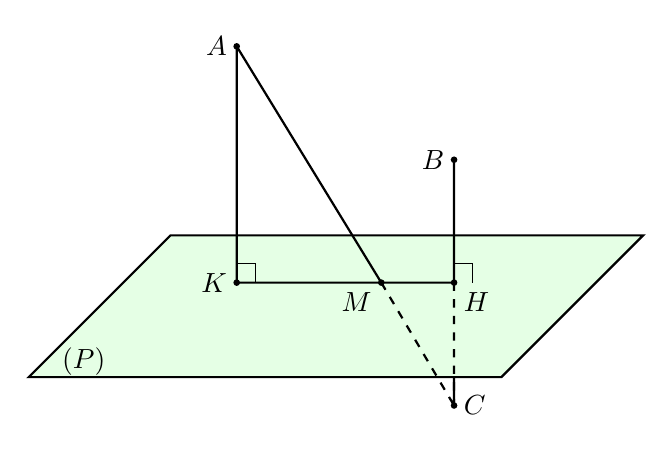
\begin{tikzpicture}[>=stealth, scale=1.2]
\coordinate (P1) at (0,0); \coordinate (P2) at (5,0);
\coordinate (P3) at (6.5,1.5); \coordinate (P4) at (1.5,1.5);
\coordinate (K) at (2.2, 1); \coordinate (H) at (4.5, 1);
\coordinate (A) at (2.2, 3.5); \coordinate (B) at (4.5, 2.3);
\coordinate (C) at (4.5, -0.3); \coordinate (M) at (3.73, 1); 
\draw[thick, fill=green!20, fill opacity=0.5] (P1) -- (P2) -- (P3) -- (P4) -- cycle;
\node[anchor=south west] at (P1) [shift={(0.3,-0.1)}] {$(P)$};
\draw[thick] (A) -- (K) (B) -- (H) (K) -- (H) (A) -- (M) (4.5, 0) -- (C);
\draw[dashed, thick] (M) -- (C) (H) -- (C);
\foreach \p/\pos/\txt in {A/left/A, B/left/B, C/right/C, K/left/K, H/below right/H, M/below left/M} {
\fill (\p) circle (1pt) node[\pos] {$\txt$};}
\foreach \x in {2.2, 4.5} {
\draw (\x, 1.2) -- (\x+0.2, 1.2) -- (\x+0.2, 1);}
\end{tikzpicture}
\end{center}}
\end{ex}
\begin{ex}%[2D1C2-1]
Mô hình $EOQ$ (Economic Order Quantity) được công bố năm 1913 là một công cụ quản trị vận hành dùng để xác định lượng hàng nhập kho tối ưu. Giả sử một cửa hàng thức ãn cho mèo có nhu cầu tiêu thụ hàng hóa đều đặn với tốc độ bán hảng $d=100$ hộp/ngày. Các thông số chi phí được xác định như sau
\begin{itemize}
\item $K=1\,000\,000$ đồng: chi phỉ cố định cho mỗi lần đặt hàng (phí vận chuyển, nhân công\ldots);
\item $c$ đồng/hộp: giá nhập mỗi hộp hàng (giả định không đổi và không có chiết khấu);
\item $h=500$ đồng/hộp/ngày: đơn giá lưu kho (chi phí lưu giữ một hộp hàng trong kho trong một ngày).
\end{itemize}
Gọi $Q$ (hộp) là số lượng hàng mà người bán nhập vào trong mỗi lần đặt hàng. Thời gian tiêu thụ hết
lượng hảng là $\dfrac{Q}{d}$ (ngày). Tổng chi phí cho một chu kỳ đặt hàng và tiêu thụ hết hàng là $f=K+cQ+\dfrac{hQ^2}{2d}$.
Hỏi cửa hàng nên nhập bao nhiêu hộp trong mỗi lần đặt hàng để chi phí trung bình mỗi ngày là nhỏ nhất \textit{(không làm tròn các bước trung gian, chỉ làm tròn kết quả cuối cùng tới hàng đơn vị)}?
\shortans[]{$632$}
\loigiai{
Gọi $g(Q)$ là hàm chi phí trung bình mỗi ngày. \\
Ta có công thức chi phí trung bình bằng tổng chi phí chia cho thời gian chu kỳ. Ta được
\begin{align*}
&g(Q)=\dfrac{f}{\dfrac{Q}{d}}=\dfrac{K+c Q+\dfrac{h Q^2}{2 d}}{\dfrac{Q}{d}}\\
&g(Q)=\dfrac{d}{Q}\left(K+c Q+\dfrac{h Q^2}{2 d}\right)=\dfrac{K d}{Q}+c d+\dfrac{h Q}{2}.
\end{align*}
Ta có đạo hàm
\[g'(Q)=-\dfrac{K d}{Q^2}+0+\dfrac{h}{2}.\]
Khi đó, 
\begin{eqnarray*}
& &g'(Q)=0\\
&\Leftrightarrow&-\dfrac{K d}{Q^2}+\dfrac{h}{2}=0\\
&\Leftrightarrow& \dfrac{h}{2}=\dfrac{K d}{Q^2}\\
&\Leftrightarrow& Q^2=\dfrac{2 K d}{h}.
\end{eqnarray*}
Vì số lượng hàng nhập $Q>0$, ta suy ra $Q=\sqrt{\dfrac{2 K d}{h}}$.\\
Thay các số liệu đã cho từ đề bài $d=100$, $K=1\,000\,000$, $h=500$ vào công thức vừa tìm được
\[
Q=\sqrt{\dfrac{2 \cdot 1\,000\,000 \cdot 100}{500}}=\sqrt{\dfrac{200\,000 \,000}{500}}=\sqrt{400\,000} \approx 632{,}4555 \ldots
\]
Theo yêu cầu của đề bài là chỉ làm tròn kết quả cuối cùng tới hàng đơn vị, ta có $Q \approx$ $632$.\\
Cửa hàng nên nhập $632$ hộp trong mỗi lần đặt hàng để chi phí trung bình mỗi ngày là nhỏ nhất.}
\end{ex}
\begin{ex}%[1D6V4-6]
Trong âm nhạc, một quãng tám (Boctave) là khoảng cách âm thanh từ nốt Đô tới nốt Đồ tiếp theo, theo thứ tự từ thấp đến cao là
\begin{center}
Đô - Đô$\sharp$ - Rê - Rê$\sharp$ - Mi(E4) - Pha - Pha$\sharp$ - Sol - Sol$\sharp$ - La (A4) - La$\sharp$ - Si - Đô
\end{center}
trong đó khoảng cách giữa hai nốt liên tiếp gọi là một nửa cung (semitone). Hai nốt cách nhau $n$ nửa cung thì tỷ lệ tần số nốt cao $f_\text{nc}$ và tằn số nốt thấp $f_\text{nt}$ là $\dfrac{f_\text{nc}}{f_\text{nt}}=2^{\tfrac{x}{12}}$; cho biết tần số chuẩn cùa nốt La (A4) là $440$
Hz. Trên đàn guitar, dây số $1$ là nốt Mi(E4) đang bị chùng do thời tiết, tần số đo được hiện tại đang là $300$
Hz. Để căng lại dây đàn cho chuẩn, ta dùng núm xoay, và cứ vặn núm xoay $90^{\circ}$ thì nốt nhạc được tăng lên một nửa cung. Hỏi phải xoay núm của dây số $1$ một góc bao nhiêu độ để dây số $1$ trở về âm chuẩn \textit{(không làm tròn các buớc trung gian, chi làm tròn kết quả cuối cùng tới hàng đơn vị)}?
\shortans[]{$147$}
\loigiai{
Từ Mi (E4) đến La (A4) có
\begin{center}
Mi $\rightarrow$ Pha (1), Pha $\rightarrow$ Pha$\sharp$ (2), Pha$\sharp$ $\rightarrow$ Sol (3), Sol $\rightarrow$ Sol$\sharp$ (4), Sol$\sharp$ $\rightarrow$ La (5).
\end{center}
Vậy Mi (E4) và La (A4) cách nhau $5$ nửa cung.\\
Ta có $\dfrac{f_\text{La}}{f_\text{Mi}}=2^{\tfrac{5}{12}}$ suy ra tần số chuẩn của Mi (E4) là $f_\text{Mi}=\dfrac{f_\text{La}}{2^{\tfrac{5}{12}}}=\dfrac{440}{2^{\tfrac{5}{12}}}$ Hz.\\
Gọi $n$ là số nửa cung cần tăng để từ $300$ Hz lên âm chuẩn của Mi , ta có
\begin{eqnarray*}
& &\dfrac{f_\text{Mi}}{300}=2^{\tfrac{n}{12}}\\
&\Leftrightarrow& \dfrac{440}{300 \cdot 2^{\tfrac{5}{12}}}=2^{\tfrac{n}{12}} \\
& \Leftrightarrow& \dfrac{n}{12}=\log _2\left(\dfrac{440}{300\cdot 2^{\tfrac{5}{12}}}\right)\\
&\Leftrightarrow& n=12 \cdot \log _2\left(\dfrac{22}{15\cdot 2^{\dfrac{5}{12}}}\right).
\end{eqnarray*}
Góc xoay cần thiết là $\alpha=n\cdot 90^{\circ}=12\cdot \log _2\left(\dfrac{22}{15\cdot 2^{\tfrac{5}{12}}}\right)\cdot 90^{\circ} \approx 147^{\circ}$.
}
\end{ex}
\begin{ex}%[0D8C1-3]
Trong một cuộc thi, có $7$ thí sinh đã được xếp ngồi cố định quanh một bàn tròn và giám thị có $3$ mã đề khác nhau (giả sử số lượng đề thi của mỗi mã là nhiều tùy ý). Hỏi có bao nhiêu cách phát đề cho các thí sinh, mỗi thí sinh $1$ đề sao cho hai thí sinh ngồi cạnh nhau thì khác mã đề?
\shortans[]{$126$}
\loigiai{
Không mất tính tổng quát, tạm thời tháo bỏ ràng buộc vòng tròn để đưa về bài toán hàng ngang đơn giản hơn, sau đó tìm mối liên hệ giữa chúng.\\
Ta xây dựng công thức tổng quát cho $n$ thí sinh với $3$ mã đề
\begin{itemize}
	\item Số cách chọn mã đề cho thí sinh số $1$ là $3$ cách.
	\item Số cách chọn mã đề cho thí sinh số $2$ khác đề thí sinh số $1$ là $2$ cách.
	\item Số cách chọn mã đề cho thí sinh thứ $3$ khác đề thí sinh số $2$ là $2$ cách.
	\item Tương tự cho đến thí sinh thứ $n$ vẫn có $2$ cách chọn mã đề. 
\end{itemize}
Áp dụng quy tắc nhân ta có $A_n=3 \cdot \underbrace{2 \cdot 2 \ldots \cdot 2}_{n-1}$.\\
Ta tiến hành cuộn hàng dài lại thành vòng tròn và nhận thấy có $2$ khả năng xảy ra nhưu sau
\begin{itemize}
\item Khả năng 1: Thí sinh 1 và thí sinh $n$ mang mã đề khác nhau.\\
Khi cuộn tròn lại, vì họ khác mã đề nên hoàn toàn thỏa mãn yêu cầu của bàn tròn (hai người cạnh nhau bất kỳ đều khác mã đề). Do đó, mỗi cách xếp ở hàng ngang thuộc khả năng này chính là một cách xếp hợp lệ cho bàn tròn $n$ người. Số cách này theo định nghĩa là $u_n$.
\item Khả năng 2: Thí sinh $1$ và thí sinh $n$ mang cùng một mã đề.\\
Khi cuộn tròn lại, hai người này ngồi cạnh nhau mà lại trùng mã đề, nên cách xếp này không hợp lệ cho bàn tròn $n$ người. Tuy nhiên, ta hoàn toàn có thể đếm được nhóm không hợp lệ này bằng cách: Coi thí sinh $1$ và thí sinh $n$ gộp lại thành một vị trí duy nhất (gọi là vị trí $1'$ ). Khi đó, vòng tròn $n$ người ban đầu biến thành một vòng tròn mới chỉ có $n-1$ người và vòng tròn mới này hoàn toàn hợp lệ (vì vị trí $1'$ khác mã đề với người số $2$ và người số $n-1$ ). Do đó, số cách xếp ở hàng ngang thuộc khả năng này chính bằng số cách xếp hợp lệ của bàn tròn $n-1$ người, tức là $u_{n-1}$.
\end{itemize}
Vì mọi cách xếp trên hàng ngang $A_n$ chỉ có thể rơi vào một trong hai khả năng xung khắc trên, ta suy ra tổng số cách của hai khả năng phải bằng chính $A_n$
\[u_n+u_{n-1}=A_n\]
Suy ra công thức truy hồi
\[u_n=3 \cdot 2^{n-1}-u_{n-1} \quad(n \geq 3)\]
Ta tính được
\begin{itemize}
	\item Với $n=2$: $u_2 = 3 \cdot 2 = 6$.
	\item Với $n=3$: $u_3 = 3 \cdot 2^2 - u_2 = 12 - 6 = 6$.
	\item Với $n=4$: $u_4 = 3 \cdot 2^3 - u_3 = 24 - 6 = 18$.
	\item Với $n=5$: $u_5 = 3 \cdot 2^4 - u_4 = 48 - 18 = 30$.
	\item Với $n=6$: $u_6 = 3 \cdot 2^5 - u_5 = 96 - 30 = 66$.
	\item Với $n=7$: $u_7 = 3 \cdot 2^6 - u_6 = 192 - 66 = 126$.
\end{itemize}
Vậy số cách phát đề cho $7$ thí sinh ngồi quanh bàn tròn là
$u_7= 126$.
}
\end{ex}
\begin{ex}%[2D4V2-6]
Vệ tinh Van Allen Probes được phóng lên không gian để nghiên cứu các vành đai bức xạ bao quanh Trái Đất. Vệ tinh này bay theo một quỹ đạo có chu kỳ $10$ giờ-nghĩa là mỗi vòng bay quanh Trái Đất kéo dài đúng $10$ giờ. Cứ mỗi vòng bay, vệ tinh lại xuyên qua vùng bức xạ mạnh và tích lũy thêm\textit{ liều bức xạ}. Biết rằng đơn vị của bức xạ là Gray (Gy) và khi tổng liều bức xạ chiếu vào vệ tinh đạt $1\,000$ Gray thì vệ tinh hỏng hoàn toàn. Khoảng cách từ tâm Trái Đất đến vệ tình được mô hình hóa bằng hàm số $R(T)=7\,000+3\,000T$ (km), trong đó $T$ là thời gian tính bằng giờ, $0\leq T\leq 10$, kể từ đầu vòng bay. Công thức \textit{suất liều bức xạ}-tức là lượng bức xạ vệ tinh nhận được trong $1$ giờ, phụ thuộc vào khoảng cách $R$ (km) từ vệ tính tới tâm Trái Đất, là $D(R)=60\cdot\left(\dfrac{R}{25\,000}\right)^2$ milliGray/giờ. Biết rằng do tính đối xứng và chu kỳ của quỹ đạo bay, tổng liều bức xạ vệ tịnh nhận được trong một vòng bay $10$ giờ được tính bằng công thức $L=2\cdot \displaystyle\int\limits_0^5 D(R(T)) \mathrm{\,d}T$ và 1 Gray $=1\,000$ milliGray. Tính số nãm hoạt động của vệ tinh từ lúc bắt đầu hoạt động tới khi hỏng hoàn toàn \textit{(không làm tròn các buớc trung gian, chi làm tròn kết quả cuối cùng tới hai chũ số thập phân sau dấu phấy, coi một năm có $365$ ngày, mỗi ngày có $24$ giờ)}.
\shortans[]{$5{,}19$}
\loigiai{
Suất liều bức xạ theo thời gian $T$ trong một vòng bay
\[
D(R(T))=60 \cdot\left(\dfrac{7\,000+3\,000 T}{25\,000}\right)^2=\dfrac{60}{625} \cdot(7+3 T)^2 \text {(milliGray/giờ)}.\]
Liều bức xạ nhận được trong một vòng bay
\[
L=2 \displaystyle\int\limits_0^5 \dfrac{60}{625}(7+3 T)^2 \mathrm{\,d}T=\dfrac{5496}{25} \text {(milliGray/vòng)}.\]
Tổng liều giới hạn $1\,000$ Gray=$1\,000\,000$ milliGray.\\
Tổng số vòng bay tối đa \[N=\dfrac{1\,000\,000}{\dfrac{5\,496}{25}}=\dfrac{25\cdot 10^6}{5\,496}\,\text{vòng}.\]
Tổng số giờ hoạt động $H=N\cdot 10=\dfrac{25\cdot 10^7}{5\,496}$ giờ.\\
Số năm hoạt động $Y=\dfrac{H}{24\cdot 365}=\dfrac{\dfrac{25\cdot 10^7}{5\,496}}{24\cdot 365} \approx 5{,}19$ năm.}
\end{ex}
\begin{ex}%[1H8V5-3]
Cho hình lăng trụ $ABC.A'B'C'$ có đáy $ABC$ là tam giác đều cạnh bằng $2$, hình chiếu của $A'$ trên trùng với trung điểm $M$ của $AB$; góc giữa cạnh bên và mặt đáy bằng $60^{\circ}$. Gọi $N$ là trung điểm của $CC'$. Tính khoảng cách từ $B'$ tới mặt phẳng ($A'MN$) \textit{(không làm tròn các bước trung gian, chỉ làm tròn kết quả cuối cùng tới hàng phần trăm)}.
\shortans[]{$1{,}92$}
\loigiai{
\begin{center}
\begin{tikzpicture}[scale=1.2, >=stealth, line join=round, line cap=round]
\coordinate (A) at (0,0);
\coordinate (B) at (1.5,-1);
\coordinate (C) at (4,0);
\coordinate (D) at (9,0);
\coordinate (vv) at (0.5, 3.5);
\foreach \p/\pp in {A/Ap, B/Bp, C/Cp} \coordinate (\pp) at ($(\p)+(vv)$);
\coordinate (M) at ($(A)!0.6!(B)$);
\coordinate (N) at (intersection of Ap--D and C--Cp);
\coordinate (E) at ($(B)!0.3!(D)$);
\coordinate (I) at ($(Ap)!0.7!(M)$);
\draw[dashed, thick] (A) -- (D) (C) -- (N) (Ap) -- (N) (A) -- (E) (M) -- (E) (B) -- (C);
\draw[thick] (Ap) -- (Bp) -- (Cp) -- cycle 
(A) -- (B)
(Ap) -- (A) (Bp) -- (B) (Cp) -- (N) 
(Ap) -- (M) (N) -- (D) (B) -- (D);
\foreach \p/\pos/\txt in {
A/left/A, B/below/B, C/below/C, D/right/D, 
M/below/M, N/right/N, E/below/E, I/right/I,
Ap/left/A', Bp/above/B', Cp/right/C'} {
\fill[blue] (\p) circle (1pt);
\node[\pos, font=\scriptsize] at (\p) {$\txt$};
}
\end{tikzpicture}
\end{center}
Gọi $I=AB' \cap A'M$ và $D=A'N \cap AC$.\\
Ta có $\dfrac{IA}{IB'}=\dfrac{1}{2}$ nên suy ra $\mathrm{d}\left(B',(AMN)\right)=2 \mathrm{d}\left(A,\left(A'MN\right)\right)$.\\
Mặt khác, theo giả thiết
\[\heva{&A'M \perp(ABC)\\&A'M \subset\left(A'MD\right)} \Rightarrow (A'MD)\perp (ABC)=MD.\]
Kẻ $AE \perp MD$.\\
Suy ra $AE=\mathrm{d}\left(A,\left(A'MD\right)\right)$.\\
Xét tam giác $A'AD$, có $\dfrac{CD}{AD}=\dfrac{CM}{AA'}=\dfrac{1}{2} \Rightarrow CD=\frac{1}{2} AD$.\\
Do đó $AC=CD=2$.\\
Mặt khác, $MD^2=AM^2+AD^2-2AM \cdot AD \cdot \cos \widehat{MAD}=13 \Rightarrow MD=\sqrt{13}$.
\[\Rightarrow S_{\triangle A'MD}=\dfrac{1}{2} \cdot AM \cdot AD \cdot \sin \widehat{MAD}=\dfrac{1}{2} \cdot 1 \cdot 4 \cdot \dfrac{\sqrt{3}}{2}=\sqrt{3}.
\]
Suy ra, 
\begin{align*}
& \mathrm{d}\left(A,\left(A'MD\right)\right)=AE=\dfrac{2 \cdot S_{\triangle AMD}}{MD}=\dfrac{2 \sqrt{3}}{\sqrt{13}}\\
\Rightarrow & \mathrm{d}\left(B',(AMN)\right)=\dfrac{4 \sqrt{3}}{\sqrt{13}} \approx 1{,}92.
\end{align*}}
\end{ex}
\Closesolutionfile{ans}

%\indapan{6}{ans/ans-11-26-2-QuangNinh-SoGD-L1-LC}
%\indapan{3}{ans/ans-11-26-2-QuangNinh-SoGD-L1-DS}
%\indapan{6}{ans/ans-11-26-2-QuangNinh-SoGD-L1-KQ}
